%\documentclass[a4paper,10.5pt]{report}
\documentclass[a4paper,10.5pt]{article}
\makeindex
\usepackage{booktabs}
\usepackage{epsfig}
\usepackage{graphicx}
\usepackage{epstopdf}
\usepackage{amsmath}
\usepackage{rotating}
\usepackage{caption}

% Title Page
\textwidth 15 true cm
\textheight 25 true cm
%\headheight  14pt
%\headsep    16pt
%\footskip   27pt
%\marginparsep 10pt
%\marginparwidth  100pt
\def\marginset#1#2{
\setlength{\oddsidemargin}{#1}
\iffalse
\reversemarginpar
\addtolength{\oddsidemargin}{\marginparsep}
\addtolength{\oddsidemargin}{\marginparwidth}
\fi

  \setlength{\evensidemargin}{0mm}
\iffalse
\addtolength{\evensidemargin}{\marginparsep}
\addtolength{\evensidemargin}{\marginparwidth}
\fi

  % \paperwidth = h + \oddsidemargin+\textwidth+\evensidemargin + h
\setlength{\hoffset}{\paperwidth}
\addtolength{\hoffset}{-\oddsidemargin}
\addtolength{\hoffset}{-\textwidth}
\addtolength{\hoffset}{-\evensidemargin}
\setlength{\hoffset}{0.5\hoffset}
\addtolength{\hoffset}{-1in}           % h = \hoffset + 1in

  \setlength{\voffset}{-1in}             % 0 = \voffset + 1in
\setlength{\topmargin}{\paperheight}
\addtolength{\topmargin}{-\headheight}
\addtolength{\topmargin}{-\headsep}
\addtolength{\topmargin}{-\textheight}
\addtolength{\topmargin}{-\footskip}
\addtolength{\topmargin}{#2}
\setlength{\topmargin}{0.5\topmargin}
}

\marginset{10mm}{12mm}
\title{E08014 Cross Section Extraction}
%\subtitle{A note of $x>2$ cross section extraction package}
\author{Zhihong Ye\\ University of Virginia}

\begin{document}
\maketitle

\section{Instruction}

 The complete process of an electron scattering is that: the electron is accelerated by CEBAF upto near 3.356 GeV and sent into Hall A, and hits on a nucleus in a target, which is stored inside a vacuum chamber, locating at the center of the hall; then the scattered electron comes out from the chamber and enter into one of two HRS (QQDQ spectrometer systems) at a specific angle, and is bended up toward the detector huts on top of HRS; when the electron comes out from HRS, it passes through two vertical drifting chambers (VDC), each of which includes two wire planes, and leaves tracks for reconstruction of its position and direction, as well as its momentum. Timing signal produced by two scintilator planes (S1 and S2m) when the electron flying thought will be used to form DAQ triggers as well as saved as TDC spectra for future Time Of Fly analysis. A gas Cherenkov detector box is located in between S1 and S2m to collect signal from Cherenkov light which is produced by the electron traveling inside, and the 
sum of the signals would directly gives the energy of the electron after calibrations; two layers of lead glasses blocks are placed behind S2m to act as Electromagnetic Calorimeter, where the electron releases its energy in form of electromagnetic cascade, or called shower.

For a group of data collected by the DAQ system and stored in one or more raw data (or a list of run numbers), we need to identify good electron events, determine the percentage of scattered electrons lost because of pre-scaling, dead time, tracking reconstruction, detectors' detection efficiencies, and particle identification cuts. 

Besides the experimental event selections, studies of acceptance effect and bin-centering corrections are performed by using Single Arm Monte Carlo simulation tool, SAMC, and cross section model, XEMC.

With all information collected above, and acceptance cuts and binning methods determined, we can proceed to calculate the cross sections. The formula of cross section as a function of $x_{bj}$ is written as following:

\begin{equation}
 \frac{d\sigma}{d\Omega dE'}(x_{bj}^{i}) = \frac{N_{EX}^{i} \epsilon_{pion\_rej}}{N_{tg} N_{e} \epsilon_{det} \epsilon_{track}} \frac{N_{MC}^{gen}}{N_{MC}^{i} \Delta\Omega_{MC} \Delta E'_{MC}}
\end{equation}

\begin{figure}[h!]
\centerline{\psfig{figure=figures/XS_Chart.pdf,scale=0.7,angle=0,clip=,keepaspectratio}}
\caption[Basic structure of the cross section extraction package]{\footnotesize{Basic structure of the cross section extraction package}
\label{xs_chart}}
\end{figure}

The absolutely cross section values are meaningless unless we understand well the systematic errors and statistic errors of the experiment. A detail discussion of errors evaluation will also be discussed.

A package of inclusive electrons scattering cross section extraction has been developed for E08-014 experiment data. The basic structure of the code and files can be viewed from the chart bellow, and a detail discussion of each step will be discussed in the next section.

\section{Extracting Cross Section}

\subsection{Beam Charge}
Base on the work on BCM calibration described in section xxx, we are able to calculate total electron charge or the total number of electrons delivered from beam in one run using equation xxx. However, if we remove events taking during beam trip, the amount of electron charge accumulated at beam currents lower than requesting values will need to be subtracted. A script was written to calculate charge and current in between two consecutive scaler events, for example, the charge and current calculated base on beam charge monitor $U_{1}$ for $ith$ scaler event are given by:

\begin{equation}
  \Delta C_{i}^{U_{1}} = C_{i+1}^{U_{1}} - C_{i}^{U_{1}},  I_{i}^{U_{1}} = \Delta C_{i}^{U_{1}}/(T_{i+1}-T_{i}),
\end{equation}

where $\Delta C_{i+1}^{U_{1}}$ gives the calibrated values of charge accumulated between two consecutive scaler events at CPU clock $(T_{i+1}$ and $T_{i})$, of which the difference is normally set to be three seconds. We assign the average value of charge and current from $U_{1}, U_{3}, D_{1}$ and $D_{3}$ to all electron scattering events happening during this time window. Then a beam trip cut will throw away events with currents lower than the cut value. And the total number of electrons from beam in one run is re-evaluated:

\begin{equation}
  N_{e} = \sum_{i^{*}} \Delta C_{i^{*}}^{avg}(I_{i^{*}}^{avg}>I_{beam\_trip\_cut}) 
\end{equation}

where the star on $i^{*}$ means summarizing scaler events with beam current $I_{i^{*}}$ higher than the cutting value $I_{beam\_trip\_cut}$, the value of which we chose to be half of the values we requested during the experiment.

During the experiment, Left BCM scalers did not work properly so we used the values of charge calculated from HRS-R BCM for HRS-L data since two arm shared the same DAQ system. 

\subsection{Targets}
Total number of scattering centers (or nuclei) in a target with specific thickness is given by:

\begin{equation}
 N_{tg} = \frac{\rho\cdot l \cdot N_{a}}{A},
\end{equation}

where $\rho$ is the target density in $g/cm^{3}$, $l$ is the target length in cm, $N_{a}$ is the Avogadro's number and A is the nuclear number of the target. 

For cryogenic long targets, such as $^{2}H, ^{3}He3 and ^{4}He3$ used in this experiment, $l$ should be equal to the range of vertex we cut, instead of the design lengths, and the densities are needed to be corrected for boiling effects:

\begin{equation}
  \rho_{cor} = \rho \cdot (1.0 - B \cdot I /100); 
\end{equation}

where $I$ and $B$ are the value of beam current and the boiling factor for a specific target, respectively. To obtain the boiling factors for each target, we took a series of Quasi-Elastic runs using different currents for each target, and fit the correlations of yields and currents. Study of boiling effect is performed by Patrica Solvignon %\ref{boiling_patricia}. 

Add the discussion of long target bumps here ...

\subsection{Live Time}

To reduce dead time when DAQ writing events into hard disks, pre-scale factors were assigned to each trigger type to control event rates. The values of pre-scale factors are stored into data stream for each run and can be read out to calculate the actually total number of events from different types. Since the values of pre-scale factors for each run may not be he same, events from each run are needed to be calculated individually before they add up together:

\begin{equation}
  N_{T_{i}}^{total} = \sum_{r} N_{T_{i}}^{r} PS^{r}(T_{i})
\end{equation}

where $N_{T_{i}}$ is the total number of events from trigger type $T_{i}$, $N_{T_{i}}^{r}$ is the total number of pre-scaled events from trigger type $T_{i}$ in run $r$ after cutting out beam trip, and $PS^{r}(T_{i})$ is the pre-scale factor of this trigger type in this run.

The total number of events calculated is needed to further corrected by detector and electronic dead time, where the later one is mainly contributed by computer dead time - an event is not recorded when the DAQ is writing another event that comes earlier. However, the trigger induced by this event is still counted by Scalers. The values of dead time, or another corresponding values, live time, can be evaluated by taking the ratio of number of events recorded by DAQ and number of counts by scalers for one specific trigger type in one run:

\begin{equation}
  LT = \frac{N_{T_{i}}^{DAQ} PS(T_{i})}{N_{T_{i}}^{Scaler}}
\end{equation}

where $N_{T_{i}}^{DAQ}$ and $N_{T_{i}}^{Scaler}$ are total number of DAQ events and scaler counts in one run after removing events taking during beam trip. And the total number of events for a list of runs is given by:

\begin{equation}
  N_{T_{i}}^{total} = \sum_{r} N_{T_{i}}^{r} PS^{r}(T_{i})/LT^{r}
\end{equation}

Note that the total number of events will be further reduced by applying different types of cuts, which will be discussed in next section.

\subsection{Events Selections}
  


\subsection{Efficiencies}
%Check in analysis_effi.tex
Detectors are not in 100\% of performance and the inefficiencies of detectors caused by hardware and software are needed to be evaluated corrected for cross section calculation. 

\subsubsection{Triggers}

 There are mainly three aspects that determine the trigger efficiency~\cite{R_Bock}, first one of which is the trigger algorithm designed to compromise between highly reducing background and keeping most of good events, second one of which would be the dead time caused by electronics and performance of detectors involved in the trigger system, and the last one of which is the writing speed of computer systems. It is important to avoid double counting detectors' inefficiencies when evaluating trigger efficiencies. The definition of trigger efficiency generally includes the inefficiency of scintillator counters and the formula is written as:

\begin{equation}
 \epsilon_{trigger\_eff} = \frac{PS1(3)\times N_{T1(3)}}{PS1(3) \times N_{T1(3)}+PS2(4)\times N_{T2(4)}},
 \label{trigger_eff}
\end{equation}

where $N_{T1(2,3,4)}$ is number of events triggered by T1(2,3,4) after prescaled by PS1(2,3,4). Tranditionally in Hall-A T1(3) is designed by requesting coincidence trigger signals between S1 and S2m, while T2(4) includes signals from GC in the trigger, which should carry the inefficiency effect of GC. However, during the E08014 experiment, T1(3) was modified to include GC signals in trigger, so the detection inefficiency of GC is canceled from the equation. Fig ~\ref{trig_eff} shows that the trigger efficiencies of our data on both arm were better than 99\%.

%\clearpage
\begin{figure}[h!]
\centerline{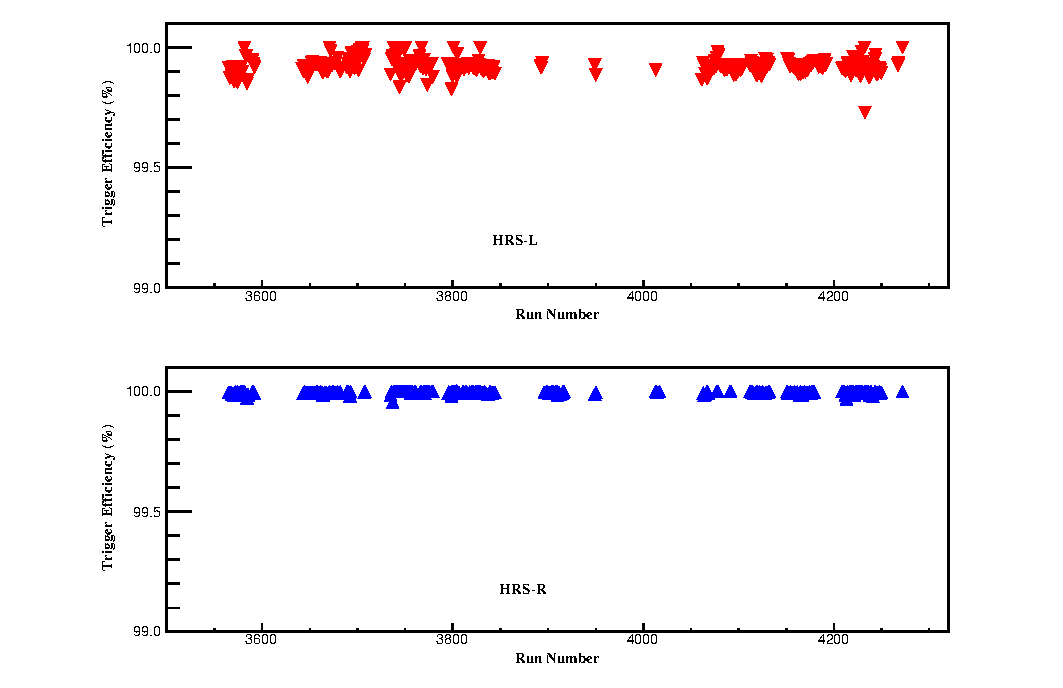
\includegraphics[width=0.7\linewidth]{figures/scin/Trigger_Eff.eps}}
\caption[Trigger Efficiencies]{\footnotesize{Trigger Efficiencies}}
\label{trig_eff}
\end{figure}

\subsubsection{VDCs}

Inefficiency of VDCs caused by hardware is neglectable and the majore source is from the misreconstruction of particle tracks during the tracking algorithm. Only one-track events are kept for analysis, and the good events threw away by zero-track and multi-tracks cut are corrected by the one-track efficiency defined as:

\begin{equation}
 \epsilon_{one\_track\_eff} = \frac{N_{Track=1}}{N_{0<=Tracks<=4}}
\end{equation}

 It is very important to select correct electron samples when calculating values of one-track efficiency. We need to avoid applying cuts on variables that require trakcing information, such as variables at focal plane and target plane, and cuting on other VDC variables will introduce other sources of inefficiencies. Cluster-reconstructed variables of calorimeters, such as E/P, can not be used when cutting electrons. cosmic ray events should also be removed since they come with big angles. We could not cut on TOF $\beta$ to suppress cosmic ray background due to the TDC multi-peaks issues on some scintillator bars. During the analysis, we used quasi-elastic carbon data which has low cosmic ray backgound due to the high rates,then applied cut on T1(3) trigger, GC ADC sum and Calorimeters ADC sum to select pure electron events, and we also require only one-hit on each scintillator bar for each event to remove events with multi-particles.From Table~\ref{vdc_table}, we obtained the fraction of one-track and multi-track events, which are above 99\% on each arm.

\begin{table}[h!]
\centering
\begin{tabular}{|c||ccccc|}
	\hline
\textbf{Number of tracks}  & 0 & 1 & 2 & 3 & 4     \\
	\hline \hline
HRS-L   & 0.0298\% & 99.1750\% & 0.7430\% & 0.0452\% & 0.0048\%  \\
        \hline
HRS-R   & 0.0482\% & 99.3600\% & 0.5446\% & 0.0388\% & 0.0073\%  \\
	\hline \hline
\end{tabular}
\caption{Fraction of different tracks events from quasi-elastic data,w/o $\beta$ cut}
\label{vdc_table}	
\end{table}

\subsubsection{PID detectors}
%\subsubsection{Gas Cherenkov}

For Gas Cherenkov detectors and lead-glass Calorimeters, there are two parts of information needed to be extracted: the fractions of particles detected when they pass throught the detectors and leave signals, or called detection efficiencies; and the percentages of electrons remaining and pions contaiminating when applying PID cuts, also called PID-Cut efficiencies. PID-Cut efficiencies basically tangle with detection efficiencies due to the fact that we deal with detected events. We need to firstly evalute detection efficiencies and PID-Cut efficiencies will be discussed in next section. 

Detection efficiency of GC (Calorimeters) can be defined as:

\begin{equation}
 \epsilon_{detection\_eff}^{cer(calo)} = \frac{N_{detected}^{cer(calo)}}{N_{samples\_from\_calo(cer)}}
\end{equation}

where $N_{cer(calo)}$ is number of particles detected by GC (Calorimeters), and $N_{samples}$ is number of particle samples from Calorimeters (GC). During the analysis, we cut on T1(3) trigger and spectrometer acceptance, and pure electron were selected by applying cuts on main peaks of E/P spectra of Calorimeters when studying GC, or on the peaks of Cherenkov ADC Sum when studying Calorimeters. 

The design of Hall A Gas Cherenkov detectors should give high detection efficiency, since electrons can easily trigger the detectors with very low threshold, while pions and other particles from cosmic ray can not fire the detectors directly, and the inefficiency is caused by particles hitting the edges of gas boxes or PMT tubes. Fig ~\ref{cer_det_eff} shows that on both arm, the detection efficiencies of Gas Cherenkov detectors are close to 100\%.

%\clearpage
\begin{figure}[h!]
\centerline{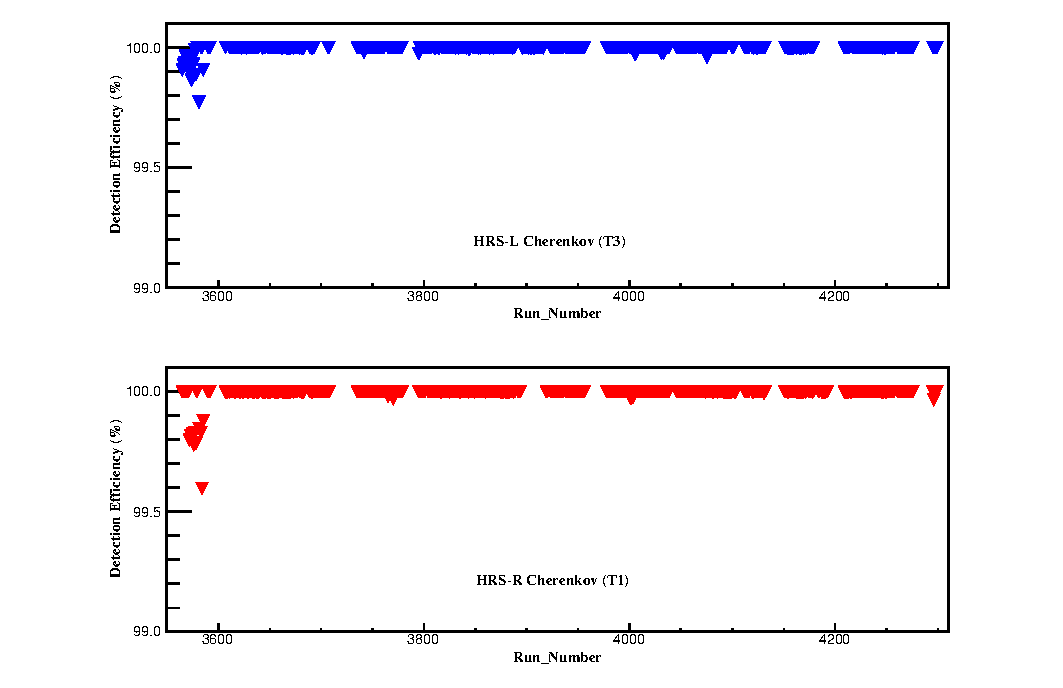
\includegraphics[width=0.7\linewidth]{figures/cer/Cer_Det_Eff.eps}}
\caption[Gas Cherenkov Detection Efficiency]{\footnotesize{Gas Cherenkov Detection Efficiency}}
\label{cer_det_eff}
\end{figure}

%\subsubsection{Calorimeters}
The detection efficiencies of lead glass calorimeters are expected to be lower than Gas Cherenkov detectors. Calorimeters are composed by piles of lead glass blocks, so the inefficiency of detection is mainly from particles going through gaps in between blocks or hitting the edges or PMT tubes before cascade. Cluster reconstruction when calculating deposited energy in lead glass blocks is another source of inefficiencies, especially when the electron rate is low and many low energy cosmic ray particles mix in.From Fig ~\ref{calo_det_eff}, we see that the detection efficiencies of calorimeters on both arm are still high than 99\% for most of runs, but for some runs with low electron rates, mainly for $^{3}He$ target with low beam current (Fig~\ref{calo_det_eff_mom}),the detection efficiencies are slightly lower, due to more cosmic ray contamination. Events from cosmic ray will eventually be removed by applying accpetance cuts and PID cuts, so no correction is necessary for those runs.  

\begin{figure}[h!]
 \centerline{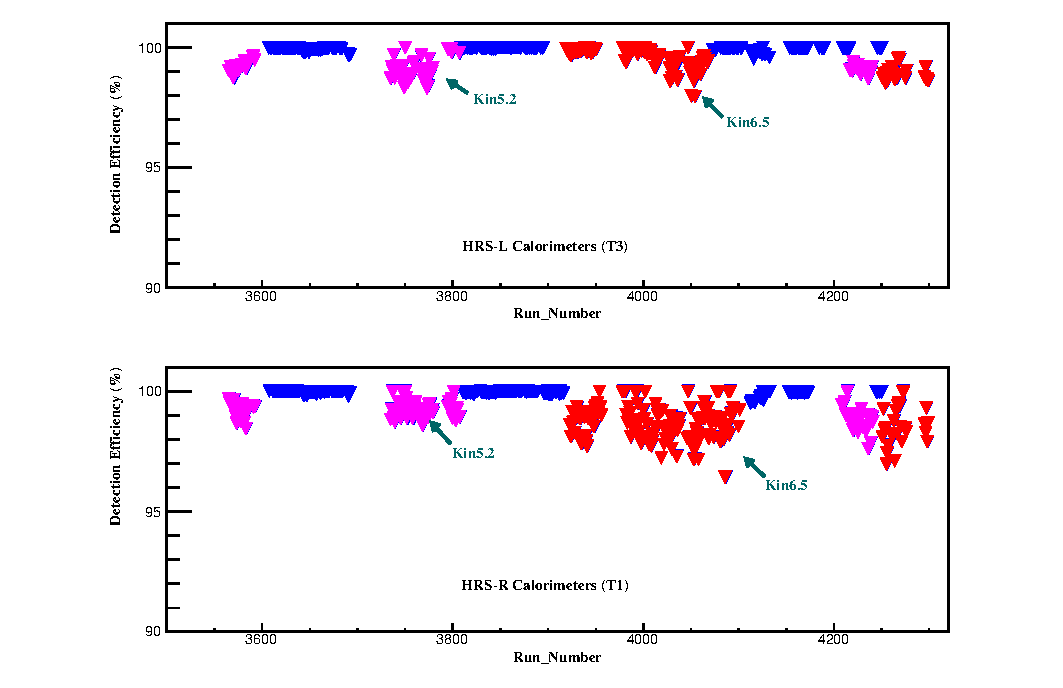
\includegraphics[width=0.7\linewidth]{figures/calo/Calo_Det_Eff1.eps}}
 \captionof{figure}{\footnotesize{Calorimeters: Efficiencies vs Run Number}}
 \label{calo_det_eff}
\end{figure}

\begin{figure}[h!]
 \centerline{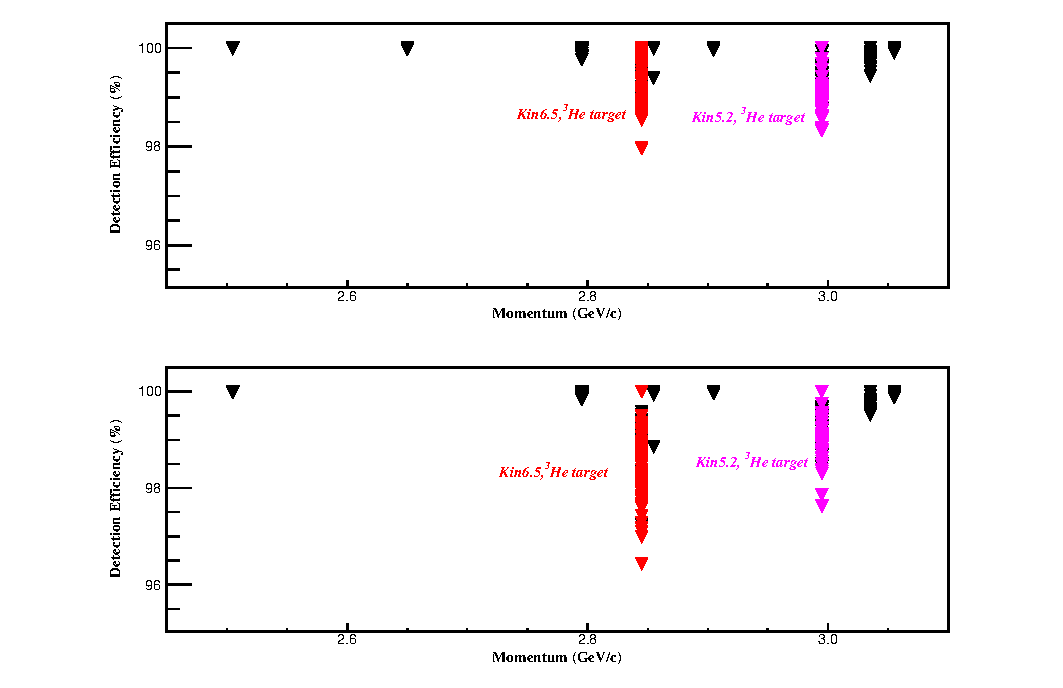
\includegraphics[width=0.7\linewidth]{figures/calo/Calo_Det_Eff_Mom1.eps}}
 \captionof{figure}{\footnotesize{Calorimeters: Efficiency vs Momentum}}
 \label{calo_det_eff_mom}
\end{figure}


\subsection{Monte Carlo Simulation}
A simulation package, Hall-a Single Arm Monte Carlo (SAMC), which was originally developed in FORTRAN by A. Deur \cite{•} and then converted into C++ by Huan Yao \cite{}, is used for study of acceptance effect and corrections.

\subsection{Cross Section Model}


\subsection{Acceptance and Binning}

\subsection{Evaluation of Errors}

\subsection{Cross Section Results}

\subsection{Discussion and Conclusion}



\end{document}

